% Introdução

\documentclass[Tese.tex]{subfiles}

\begin{document}
	
\chapter{Modelo numérico de contato}\label{ch:contato}

O modelo de contato descrito neste capítulo é uma extensão do modelo aplicado em \citeonline{Pericles2019}, onde foi utilizado o método nó-a-segmento em conjunto com multiplicadores de Lagrange para problemas bidimensionais. Neste trabalho, considera-se também o caso tridimensional, demandando o emprego de uma estratégia nó-a-superfície. Além disso, algumas modificações gerais são feitas ao modelo original de forma a melhorar sua precisão, entre elas:
\begin{itemize}[itemsep=-0.8ex]
	\item A detecção do contato é feita por meio da intersecção das trajetórias dos elementos, ao invés do ponto de mínima distância. Essa modificação é pouco importante no caso sem atrito, onde o ponto original de contato não possui grande influência no ponto final após o deslizamento. No entanto, para o caso com atrito, é importante garantir que a condição de aderência seja aplicada no ponto correto, onde ocorreu originalmente o contato.
	\item As coordenadas adimensionais dos pontos de contato são adicionadas como parâmetros do sistema global, sendo recalculadas a cada iteração pelo método de Newton-Raphson, juntamente com as posições e os multiplicadores de Lagrange. No método original, os pontos de contato eram permitidos deslizar apenas transversalmente ao ponto original, o que poderia causar inconsistências em elementos de alta ordem (especialmente elementos com certo grau de curvatura), pois o nó projétil poderia acabar fora do domínio dos elementos alvo. Para contornar esse problema, os pontos de contato eram atualizados ao final de cada convergência do Newton-Raphson, e o sistema era calculado novamente com os novos pontos, gerando mais iterações e comprometendo a ordem de convergência. Já no presente modelo, pelo fato de as coordenadas adimensionais serem atualizadas a cada iteração, o ponto de contato é permitido deslizar apenas dentro do próprio domínio do elemento, evitando as inconsistências mencionadas previamente e reduzindo a necessidade de refazer o processo de Newton-Raphson em cada passo de tempo. Apesar disso, o novo modelo possui a desvantagem de apresentar um tempo de processamento maior em cada iteração, devido à introdução de parâmetros adicionais, aumentando a ordem do sistema.
\end{itemize}

\section{Discretização do contato pela estratégia nó-a-superfície}\label{sec:disc-contato}

No método nó-a-superfície, os pares de interface de contato distinguem-se entre ``projéteis'', onde os elementos de contato são os nós, e ``alvos'', onde os elementos de contato são as superfícies (ou segmentos, no caso 2D). Esses últimos utilizam como base a malha do sólido, sendo discretizados por elementos finitos de superfície (neste trabalho, triangulares ou quadrilaterais), ou de linha no caso 2D.  Dessa forma, pode-se escrever as posições ao longo de uma superfície pela interpolação:
\begin{equation}\label{eq:yS}
\yS(\coords) = \fforma\nodeind(\coords)\y\nodeind,
\end{equation}
onde o índice $\node$ é somado por todos os nós do elemento alvo, e $\fforma\nodeind$ denota a função de forma desse elemento aplicada ao nó $\node$, que depende, neste caso, das coordenadas adimensionais $\coords$. Derivando $\yS$ com relação à cada componente de $\coords$, temos os vetores tangentes e tangentes unitários, definidos, respectivamente, pelas expressões:
\begin{align}
&\tang^i(\coords) = \dfrac{\partial\fforma\nodeind}{\partial\coordsind_i}\y\nodeind, \quad\text{e}\\
&\tangun^i(\coords) = \tang^i/\|\tang^i\|.
\end{align}
Observa-se que no caso 3D há dois vetores tangentes ($i=1$, $i=2$), enquanto no caso 2D apenas um ($i=1$). O vetor normal, denotado por $\normal$, é calculado de forma que $\normal\cdot\tangun^i = 0$ para cada $i$. No caso 3D, ele é o produto vetorial entre os dois vetores tangente, isto é,
\begin{equation}\label{eq:normal3D}
\normal = \tangun^1 \times \tangun^2.
\end{equation}
No caso bidimensional, a mesma regra se aplica, porém considerando $\tangun^2 = (0,0,1)$, o que resulta simplesmente em
\begin{equation}\label{eq:normal2D}
\normalind_1 = \tangunind^1_2 \text{\qquad e\qquad} \normalind_2 = -\tangunind^1_1.
\end{equation}
O vetor normal 2D calculado pela \autoref{eq:normal2D} será automaticamente unitário. Já o vetor normal 3D calculado pela \autoref{eq:normal3D} pode ter norma diferente de $1$. Nesse caso, calcula-se o vetor normal unitário por
\begin{equation}
\normalun = \normal/\|\normal\|.
\end{equation}

Nota-se que o sentido de $\normal$ e $\normalun$ irá depender da orientação do elemento finito. Para padronizar as equações posteriores, convenciona-se neste trabalho que os vetores normais apontam para fora do sólido. No caso 2D, isso pode ser obtido orientando os elementos de linha no sentido anti-horário em contornos externos do sólido, e sentido horário em contornos internos (como furos). No caso 3D a orientação dos elementos finitos irá depender do algoritmo de geração de malha utilizado, sendo recomendável avaliar o sentido durante a criação da geometria.

\section{Detecção do contato}

Neste trabalho, ativa-se o contato em um determinado nó projétil quando a sua trajetória intersecta a trajetória de algum elemento alvo. Adotam-se, para fins de simplificação, trajetórias lineares entre os passos de tempo, isto é, estima-se a posição de um nó projétil entre os passos anterior e atual por meio da função linear
\begin{equation}\label{eq:trajetoria-yN}
\yN^{int}(\intersectionTime) = \intersectionTime\yN + (1-\intersectionTime)\yN^{s-1},
\end{equation}
onde $\yN$ e $\yN^{s-1}$ são as posições do nó projétil no passo atual e anterior, respectivamente, e $\intersectionTime$ é um parâmetro que representa o tempo adimensional decorrido entre os dois passos, valendo $0$ para o passo anterior e $1$ para o atual. Analogamente, para cada nó $\node$ de um elemento alvo, podemos estimar sua posição no tempo $\intersectionTime$ pela função
\begin{equation}
\y\nodeinddown^{int}(\intersectionTime) = \intersectionTime\y\nodeinddown + (1-\intersectionTime)\y\nodeinddown^{s-1},
\end{equation}
onde $\y\nodeinddown$ e $\y\nodeinddown^{s-1}$ são as posições do nó no passo atual e anterior, respectivamente. Assim, para um ponto qualquer do domínio do elemento alvo definido pela coordenada adimensional $\coords$, temos
\begin{equation}\label{eq:trajetoria-yS}
\yS^{int}(\intersectionTime,\coords) = \fforma\nodeind(\coords)\left[\intersectionTime\y\nodeinddown + (1-\intersectionTime)\y\nodeinddown^{s-1}\right],
\end{equation}
onde, novamente, o índice $\node$ é somado sobre todos os nós do elemento. Neste contexto, a condição de intersecção entre as trajetórias do nó projétil e do elemento alvo pode ser vista como $\mathbf{r}(\intersectionTime,\coords) = \yN^{int}(\intersectionTime) - \yS^{int}(\intersectionTime,\coords) = \mathbf{0}$. Aplicando nessa as \cref{eq:trajetoria-yN,eq:trajetoria-yS} temos, enfim:
\begin{equation}\label{eq:interseccao}
\mathbf{r}(\intersectionTime,\coords) = \intersectionTime\yN + (1-\intersectionTime)\yN^{s-1} - \fforma\nodeind(\coords)\left[\intersectionTime\y\nodeinddown + (1-\intersectionTime)\y\nodeinddown^{s-1}\right] = \mathbf{0}.
\end{equation}

A \cref{eq:interseccao} é um sistema não-linear de equações para $\intersectionTime$ e $\coords$, cuja ordem é o número de dimensões do problema, calculado neste trabalho pelo método de Newton-Raphson. De forma a obter a convergência adequada do método, utilizam-se as derivadas:
\begin{align}
& \dfrac{\partial \mathbf{r}}{\partial \intersectionTime} = \yN - \yN^{s-1} - \fforma\nodeind(\coords)\left(\y\nodeinddown -\y\nodeinddown^{s-1}\right),\\
& \dfrac{\partial \mathbf{r}}{\partial \coordsind_j} = -\dfrac{\partial \fforma\nodeind}{\partial \coordsind_j}\left[\intersectionTime\y\nodeinddown + (1-\intersectionTime)\y\nodeinddown^{s-1}\right],
\end{align}

Esse sistema é calculado para cada combinação de nó projétil e elemento alvo. Caso ocorra a convergência, verificam-se os valores de $\intersectionTime$ e $\coords$ obtidos. Naturalmente, a intersecção precisa ter ocorrido entre os passos anterior e atual, isto é, o valor de $\intersectionTime$ deve estar entre $0$ e $1$. Além disso, as coordenadas adimensionais $\coords$ precisam pertencer ao domínio do elemento finito. Caso essas condições sejam atendidas, ativa-se finalmente o contato entre o nó projétil e o elemento alvo, e o valor de $\coords$ calculado é adotado como ponto de aderência, caso haja atrito.


%Seja um nó projétil, com posição no passo atual denotada por $\yN$, e posição no passo anterior denotada por $\yN\indprev$. Ativa-se o contato nesse nó quando, para algum segmento alvo, e para alguma coordenada adimensional $\coordsind$, sua distância normal seja menor ou igual a zero, isto é
%\begin{equation}\label{eq:gN}
%\gN = \left[\yN-\yS(\coordsind)\right]\cdot\normal(\coordsind) \leq 0.
%\end{equation}
%O ponto de contato é tomado como sendo aquele com menor valor de $\gN$ em módulo. Isso ocorre nos pontos onde a distância tangente é nula, isto é
%\begin{equation}\label{eq:gT}
%\gT = \left[\yN-\yS(\coordsind)\right]\cdot\tang(\coordsind) = 0.
%\end{equation}
%A \cref{eq:gT} é, em geral, não-linear para $\coordsind$, sendo resolvida neste trabalho de forma iterativa, pelo método de Newton-Raphson.

\section{Imposição das condições de contato}

Neste trabalho, a imposição das condições de contato é feita pelo método dos multiplicadores de Lagrange, adicionados como parâmetros nodais ao sistema, associados às forças normais de contato. Além disso, conforme discutido previamente, as coordenadas adimensionais $\coords$ do ponto de contato também são introduzidas como parâmetros do sistema, gerando novas equações denominadas condições de deslizamento. Descreve-se a seguir como essa imposição é feita para os casos sem e com atrito.

\subsection{Contato sem atrito}\label{subsec:sematrito}

A condição primária de contato a ser imposta é a de impenetrabilidade, que é traduzida como $\gN\nodeind=\left(\yN\nodeind-\yS\right)\cdot\normalun=0$, onde $\gN\nodeind$ é a distância normal entre o nó projétil $\node$ e seu respectivo ponto de contato no elemento alvo. Essa condição é imposta neste trabalho pelo método dos multiplicadores de Lagrange, onde, para cada nó de contato $\node$, adiciona-se à \cref{eq:energy} (energia mecânica total) a parcela
\begin{equation}\label{eq:Picont}
\Energiacont\nodeind = \lagN\nodeind\gN\nodeind = \lagN\nodeind \left(\yN\nodeind-\yS\right)\cdot\normalun.
\end{equation}
O termo $\lagN\nodeind$, denominado multiplicador de Lagrange, é adicionado como parâmetro do sistema global, assumindo também neste contexto o significado físico de força normal de contato. 

Observa-se que ambos $\yS$ e $\normalun$ dependem das coordenadas adimensionais de contato ($\coords$) e das posições nodais do elemento alvo (denotadas por $\yS\nodeindDois$ para cada nó $\nodeDois$). Logo, $\Energiacont\nodeind$ depende de $\lagN\nodeind$, $\yN\nodeind$, $\yS\nodeindDois$ e $\coords$. Sendo assim, com o intuito de aplicar o princípio da energia mecânica total estacionária, calcula-se a variação da \cref{eq:Picont} pela expressão
\begin{equation}\label{eq:deltaPicont}
\delta\Energiacont\nodeind =\delta\lagN\nodeind\gN\nodeind + \lagN\nodeind\normalun \cdot \delta\yN\nodeind + \lagN\nodeind\dfrac{\partial\gN\nodeind}{\partial \yS\nodeindDois}\cdot \delta\yS\nodeindDois + \lagN\nodeind\dfrac{\partial\gN\nodeind}{\partial \coords}\cdot \delta\coords,
\end{equation}
onde o índice $\beta$ é somado em todos os nós do elemento alvo. Os termos da \cref{eq:deltaPicont} multiplicando as variações $\delta\yN\nodeind$ e $\delta\yS\nodeindDois$ podem ser adicionados à \cref{eq:equilibrio-mef} como forças de contato, denotadas por $\fcont\nodeind$ e $\fcont\nodeindDois$, respectivamente. Já os termos multiplicando $\delta\lagN\nodeind$ e $\delta\coords$ são igualados a zero e introduzidos como equações adicionais do sistema.

Levando em conta que $\yS = \fforma\nodeindDois\yS\nodeindDois$, a derivada parcial de $\gN\nodeind$ com relação a $\yS\nodeindDois$ pode ser calculada pela expressão
\begin{equation}
\dfrac{\partial\gN\nodeind}{\partial \yS\nodeindDois} = -\fforma\nodeindDois\normalun + \left(\yN\nodeind-\yS\right)\cdot\dfrac{\partial\normalun_{\;\;}}{\partial\yS\nodeindDois},
\end{equation}
logo, as forças de contato aplicadas no nó projétil e nos nós do elemento alvo podem ser expressas, respectivamente, como
\begin{align}
&\fcont\nodeind = \lagN\nodeind \normalun  \text{,\quad e} \label{eq:fcontN}\\
&\fcont\nodeindDois = \lagN\nodeind\dfrac{\partial\gN\nodeind}{\partial \yS\nodeindDois} = - \lagN\nodeind \fforma\nodeindDois\normalun + \lagN\nodeind \left(\yN\nodeind-\yS\right)\cdot\dfrac{\partial\normalun_{\;\;}}{\partial\yS\nodeindDois}. \label{eq:fcontS}
\end{align}
O termo da \cref{eq:deltaPicont} multiplicando $\delta\lagN\nodeind$ introduz a condição de não-penetração ao sistema, lida como
\begin{equation}
\gN\nodeind = \left(\y\nodeind-\yS\right)\cdot\normalun = 0. \label{eq:gN0}
\end{equation}
Por fim, para o cálculo do termo multiplicando $\delta\coords$, leva-se em conta que a derivada parcial de $\gN\nodeind$ com relação a $\coords$ é dada pela expressão
\begin{equation}
\dfrac{\partial\gN\nodeind}{\partial \coordsind_i} = \cancel{-\tang^i\cdot\normalun} + \left(\yN\nodeind-\yS\right)\cdot\dfrac{\partial\normalun_{\;\;}}{\partial\coordsind_i} = \left(\yN\nodeind-\yS\right)\cdot\dfrac{\partial\normalun_{\;\;}}{\partial\coordsind_i}.
\end{equation}
Vale ser dito que, para os casos em que são utilizados elementos finitos de primeira ordem, $\normalun$ é constante ao longo do elemento, logo $\partial\normalun/\partial\coordsind_i = 0$ e a parcela da \cref{eq:deltaPicont} associada à $\delta\coords$ se anula. Por esse motivo, modelos clássicos de contato com elementos lineares desconsideram a variação de $\coords$ em sua formulação, e mesmo modelos aplicados a elementos de alta ordem comumente utilizam diferentes abordagens para tratar desse problema. Em \citeonline{Pericles2019}, por exemplo, as coordenadas adimensionais são mantidas fixas, e atualizadas somente após cada processo de Newton-Raphson global, durante a verificação das mudanças de condições de contato. Já no presente trabalho, opta-se por introduzir $\coords$ como um dos parâmetros do sistema, atualizando-o a cada iteração do processo de Newton-Raphson. Dessa forma, o termo da \cref{eq:deltaPicont} multiplicando a variação $\delta\coords$ é introduzido como uma equação adicional do sistema, denominada condição de deslizamento, e lida como
\begin{equation}\label{eq:deslizamento}
\lagN\nodeind\dfrac{\partial\gN\nodeind}{\partial \coords} = \lagN\nodeind\left(\yN\nodeind-\yS\right)\cdot\dfrac{\partial\normalun}{\partial\coords} = \mathbf{0}.
\end{equation}

As \cref{eq:fcontN,eq:fcontS,eq:gN0,eq:deslizamento} constituem as parcelas do resíduo associadas ao contato sem atrito, e devem ser linearizadas com relação às posições nodais, aos multiplicadores de Lagrange ($\lagN\nodeind$) e às coordenadas adimensionais de contato ($\coords$) de forma a garantir a convergência adequada do processo de Newton-Raphson global. Uma vez que o modelo de contato implementado não conta com a possibilidade de adesão, as forças normais de contato devem ser sempre compressivas, isto é, $\lagN\nodeind < 0$. Sendo assim, a condição aplicada no algoritmo para a desativação do contato é $\lagN\nodeind \geq 0$.

\subsection{Contato com atrito de Coulomb}

Para o caso com atrito, além da força normal ($\lagN\nodeind$), considera-se, para cada nó projétil ativo $\node$, uma força transversal de contato, denotada por $\lagTvec\nodeind$. Neste trabalho, determina-se $\lagTvec\nodeind$ pela lei de Coulomb, que pode ser expressa pelas seguintes condições:
\begin{align}
&\theta = \|\lagTvec\nodeind\|-\friction|\lagN\nodeind| \leq 0, \text{\quad e}\\
&\theta\gTvec\nodeind = \mathbf{0}, \label{eq:atrito2}
\end{align}
onde $\friction$ é o coeficiente de atrito, e $\gTvec\nodeind$ é a distância tangencial do nó $\node$ ao ponto original de contato. O vetor $\gTvec\nodeind$ pode ser definido como a projeção do deslizamento total ($\gvec\nodeind$) sobre o plano tangente do elemento alvo, isto é,
\begin{equation}\label{eq:gTnode}
\gTvec\nodeind = \gvec\nodeind - \left(\gvec\nodeind\cdot\normalun\right)\normalun
\end{equation}
onde $\gvec\nodeind = \yN\nodeind-\yStick$, sendo $\yStick$ a posição original de contato, também chamada de posição de aderência (\emph{stick}). A \cref{eq:atrito2} é chamada condição de Kuhn-Tucker. A partir dela, o seguinte pode ser inferido:
\begin{enumerate}
	\item Se $\theta$ é menor que 0, isto é, se a magnitude da força transversal é menor que $\friction|\lagN\nodeind|$, então não deve haver deslizamento tangencial;
	\item Se houver deslizamento tangencial, então $\theta$ precisa ser nulo, isto é, a força transversal deve ter mesma magnitude de $\friction|\lagN\nodeind|$.
\end{enumerate}
Essas condições são chamadas, respectivamente, aderência e deslizamento, sendo tratados separadamente no modelo desenvolvido. O algoritmo implementado é baseado em etapas de previsão e correção, isto é: assume-se inicialmente condição de aderência, e calcula-se o valor de $\theta$. Se $\theta \leq 0$, a previsão está correta e a solução é mantida. Caso contrário, assume-se a condição de deslizamento. 

\subsubsection{Condição de aderência}

No caso de aderência, temos, além da condição de impenetrabilidade, uma condição de não-deslizamento, que é imposta também pelo método dos multiplicadores de Lagrange. Assim, para cada nó $\node$ em aderência, adiciona-se à energia mecânica total, além da parcela $\Energiacont\nodeind$ dada na \cref{eq:Picont}, a parcela
\begin{equation}\label{eq:Piader0}
\Energiaader\nodeind = \lagTvec\nodeind\cdot\gTvec\nodeind
\end{equation}
É importante notar que, pelo fato de $\lagTvec\nodeind$ ser uma força transversal, ela pode ser escrita de forma única como combinação linear dos vetores tangentes, isto é, $\lagTvec\nodeind = (\lagT\nodeind)^i\tangun^i$. Aplicando ainda a \cref{eq:gTnode}, e levando em conta que $\tangun^i\cdot\normalun = 0$ para todo vetor tangente $i$, temos que a \cref{eq:Piader0} pode ser reescrita simplesmente como
\begin{equation}\label{eq:Piader}
\Energiaader\nodeind = \left[(\lagT\nodeind)^i\tangun^i\right]\cdot \left[\gvec\nodeind - \left(\gvec\nodeind\cdot\normalun\right)\normalun\right] = (\lagT\nodeind)^i\tangun^i\cdot\gvec\nodeind = (\lagT\nodeind)^i(\gT\nodeind)^i,
\end{equation}
onde o índice $i$ é somado sobre todos os vetores tangente do elemento, $(\gT\nodeind)^i = \gvec\nodeind\cdot\tangun^i$ é a projeção do deslizamento sobre o vetor tangente $i$, e os termos $(\lagT\nodeind)^i$ são multiplicadores de Lagrange que representam a força transversal na direção $i$. Nota-se também que, pela condição de aderência, a coordenada adimensional de contato $\coords$ deve ser mantida fixa, e portanto sua variação não é considerada neste caso. Dessa forma, a variação da \cref{eq:Piader} pode ser escrita como
\begin{equation}\label{eq:deltaPiader}
\delta\Energiaader\nodeind = \delta(\lagT\nodeind)^i(\gT\nodeind)^i + (\lagT\nodeind)^i\dfrac{\partial (\gT\nodeind)^i}{\partial \yN\nodeind}\cdot \delta\yN\nodeind + (\lagT\nodeind)^i\dfrac{\partial (\gT\nodeind)^i}{\partial \yS\nodeindDois}\cdot \delta\yS\nodeindDois.
\end{equation}

Os termos da \cref{eq:deltaPiader} multiplicando $\delta\y\nodeind$ e $\delta\y\nodeindDois$ são adicionados à equação de equilíbrio global como forças tangenciais de aderência, expressas, respectivamente, como
\begin{align}
&\ftang\nodeind = (\lagT\nodeind)^i\dfrac{\partial (\gT\nodeind)^i}{\partial \yN\nodeind} = (\lagT\nodeind)^i \tangun^i  \text{,\quad e} \label{eq:ftangN}\\
&\ftang\nodeindDois = (\lagT\nodeind)^i\dfrac{\partial (\gT\nodeind)^i}{\partial \yS\nodeindDois} = - (\lagT\nodeind)^i \fforma\nodeindDois\tangun^i + (\lagT\nodeind)^i \gvec\nodeind\cdot\dfrac{\partial\tangun^i}{\partial\yS\nodeindDois}, \label{eq:ftangS}
\end{align}
e o termo multiplicando $(\lagT\nodeind)^i$ introduz novas equações a serem adicionada ao sistema global, denominadas condições de não-deslizamento, dadas, para cada índice $i$ de vetor tangente, pela expressão
\begin{equation}
(\gT\nodeind)^i = \left(\yN\nodeind-\yStick\right)\cdot\tangun^i = 0, \label{eq:gT0}
\end{equation}

Reitera-se que a parcela de energia referente à condição de impenetrabilidade, apresentada na \autoref{subsec:sematrito}, também deve ser incluída neste caso. Dessa forma, as \cref{eq:fcontN,eq:fcontS} (forças de contato normal) continuam sendo adicionadas à equação de equilíbrio global, e a \cref{eq:gN0} (condição de não-penetração) também é considerada no sistema. No entanto, pelo fato de não haver variação de $\coords$ neste caso, a \cref{eq:deslizamento} (condição de deslizamento) é desconsiderada.


\subsubsection{Condição de deslizamento}

Na condição de atrito com deslizamento, $\lagTvec\nodeind$ deixa de ser representada por meio de parâmetros nodais e torna-se uma força prescrita não-conservativa aplicada no nó $\node$. Conforme discutido anteriormente, pela lei de Coulomb, a magnitude de $\lagTvec\nodeind$ deve ser igual à magnitude de $\friction\lagN\nodeind$. Além disso, a direção da força é tomada contrária à direção do deslizamento. Assim, podemos escrever
\begin{equation}\label{eq:forca-atrito0}
\lagTvec\nodeind = -\friction|\lagN\nodeind|\dfrac{\gTvec\nodeind}{\|\gTvec\nodeind\|} \qquad\text{ou}\qquad (\lagT\nodeind)^i = -\friction|\lagN\nodeind|\dfrac{(\gT\nodeind)^i}{\|\gTvec\nodeind\|},
\end{equation}
para cada índice $i$ de vetor tangente. Podemos ainda aplicar o fato de $\lagN\nodeind$ ser negativo, conforme discutido previamente. Assim, $|\lagN\nodeind| = -\lagN\nodeind$, e a \cref{eq:forca-atrito0} pode ser reescrita simplesmente como
\begin{equation}\label{eq:forca-atrito}
\lagTvec\nodeind = \friction\lagN\nodeind\dfrac{\gTvec\nodeind}{\|\gTvec\nodeind\|} \qquad\text{ou}\qquad (\lagT\nodeind)^i = \friction\lagN\nodeind\dfrac{(\gT\nodeind)^i}{\|\gTvec\nodeind\|}.
\end{equation}

Neste caso, a força prescrita $\lagTvec\nodeind$ é adicionada diretamente à variação de energia mecânica total do sistema, pela parcela $\delta\Energiadesliz\nodeind = \lagTvec\nodeind\cdot\delta\gTvec\nodeind$. Como $\gTvec\nodeind$ depende de $\yN\nodeind$, $\yS\nodeindDois$ e $\coords$, podemos escrever
\begin{equation}\label{eq:deltaPidesliz}
\delta\Energiadesliz\nodeind = \lagTvec\nodeind\cdot \delta\gTvec\nodeind = \lagTvec\nodeind\cdot \dfrac{\partial \gTvec\nodeind}{\partial \yN\nodeind}\cdot \delta \yN\nodeind + \lagTvec\nodeind\cdot \dfrac{\partial \gTvec\nodeind}{\partial \yS\nodeindDois}\cdot \delta\yS\nodeindDois + \lagTvec\nodeind\cdot \dfrac{\partial \gTvec\nodeind}{\partial \coords}\cdot \delta\coords
\end{equation}
onde o índice $\beta$ é somado sobre todos os nós do elemento alvo. De forma análoga aos casos anteriores, os termos da \cref{eq:deltaPidesliz} multiplicando as variações $\delta\yN\nodeind$ e $\delta\yS\nodeindDois$ podem ser adicionados à equação de equilíbrio global como forças tangenciais de atrito, expressas, respectivamente, como
\begin{align}
&\ftang\nodeind = \lagTvec\nodeind\cdot \dfrac{\partial \gTvec\nodeind}{\partial \yN\nodeind} = \lagTvec\nodeind - \cancel{\left(\lagTvec\nodeind\cdot \normalun\right)}\normalun = \lagTvec\nodeind \text{,\quad e} \label{eq:ftangdeslN}\\
&\ftang\nodeindDois = \lagTvec\nodeind\cdot \dfrac{\partial \gTvec\nodeind}{\partial \yS\nodeindDois} = -\fforma\nodeind\lagTvec\nodeind - (\gvec\nodeind\cdot \normalun)\lagTvec\nodeind\cdot \dfrac{\partial\normalun}{\partial\yS\nodeindDois}, \label{eq:ftangdeslS}
\end{align}
onde utilizou-se o fato de que $\lagTvec$ é uma força tangente, isto é, $\lagTvec\nodeind\cdot\normalun = 0$. Já a parcela de \cref{eq:deltaPidesliz} multiplicando $\delta\coords$ é adicionada à \cref{eq:deslizamento} e igualada a zero, resultando na seguinte condição de deslizamento:
\begin{equation}\label{eq:deslizamento-atrito}
\left[\lagN\nodeind\left(\yN\nodeind-\yS\right) - (\gvec\nodeind\cdot \normalun)\lagTvec\nodeind\right]\cdot\dfrac{\partial\normalun}{\partial\coords} = \mathbf{0}.
\end{equation}

Novamente, observa-se que as forças normais de contato, dispostas nas \cref{eq:fcontN,eq:fcontS}, continuam sendo adicionadas à equação de equilíbrio global, e a condição de não-penetração, \cref{eq:gN0}, também é considerada sem modificações. É possível verificar que, neste caso, a linearização das equações resulta em uma matriz tangente não-simétrica, ao contrário dos problemas estruturais apresentados até então neste trabalho, exigindo um tratamento numérico diferenciado.

\section{Exemplos numéricos}\label{sec:contato-exemplos}

A formulação de contato descrita neste capítulo é implementada no programa desenvolvido, e aplicada a exemplos numéricos em duas ou três dimensões. A seguir, são apresentados alguns desses exemplos, com o intuito de verificar ou demonstrar as possibilidades de aplicação do algoritmo desenvolvido. São apresentados ainda exemplos adicionais de conformação de metais, baseados nos exemplos originalmente propostos por \citeonline{Pericles2019}, porém com a consideração de atrito.

\subsection{Contato entre cilindro e bloco hiperelástico}\label{subsec:contato1}

Este exemplo, proposto originalmente por \citeonline{FENG20032213}, é utilizado para verificar o algoritmo de contato (com atrito) implementado. Considera-se um cilindro rígido sujeito a deslocamento prescrito sobre um bloco hiperelástico, conforme os dados dispostos na \autoref{fig:exemploContato}. De forma a verificar as duas versões do algoritmo, o problema é analisado tanto em 2 quanto em 3 dimensões, utilizando elementos finitos quadrilaterais e hexaédricos de ordem 3 (Q16 e HEX64, respectivamente). Por conta da simetria do problema, apenas metade do domínio é discretizado, com as devidas condições de contorno aplicadas no eixo de simetria. No caso 3D, as interfaces do sólido são ainda restritas no eixo z, de forma a simular o estado plano de deformações aplicado no exemplo original. Além disso, a espessura é tomada como $10$ mm de forma a facilitar a visualização, porém, os resultados obtidos são divididos por $10$ quando aplicável, para possibilitar a comparação com o problema original, onde aplica-se espessura unitária. Com relação ao contato, as interfaces do cilindro são discretizadas como segmentos alvos, enquanto as interfaces do bloco como nós projéteis, e o coeficiente de atrito é $\friction = 0,4$. Por fim, o número de passos de tempo adotado é $100$.

\begin{figure}[!htb]
	\centering
	\caption{Dados do exemplo de contato entre cilindro e bloco hiperelástico}
\label{fig:exemploContato}
	{\small
		\noindent\shadowbox{
			\parbox{15.3cm}{
				\setlength{\columnseprule}{1pt}
				\vspace{-0.2cm}
				{\centering\begin{center}	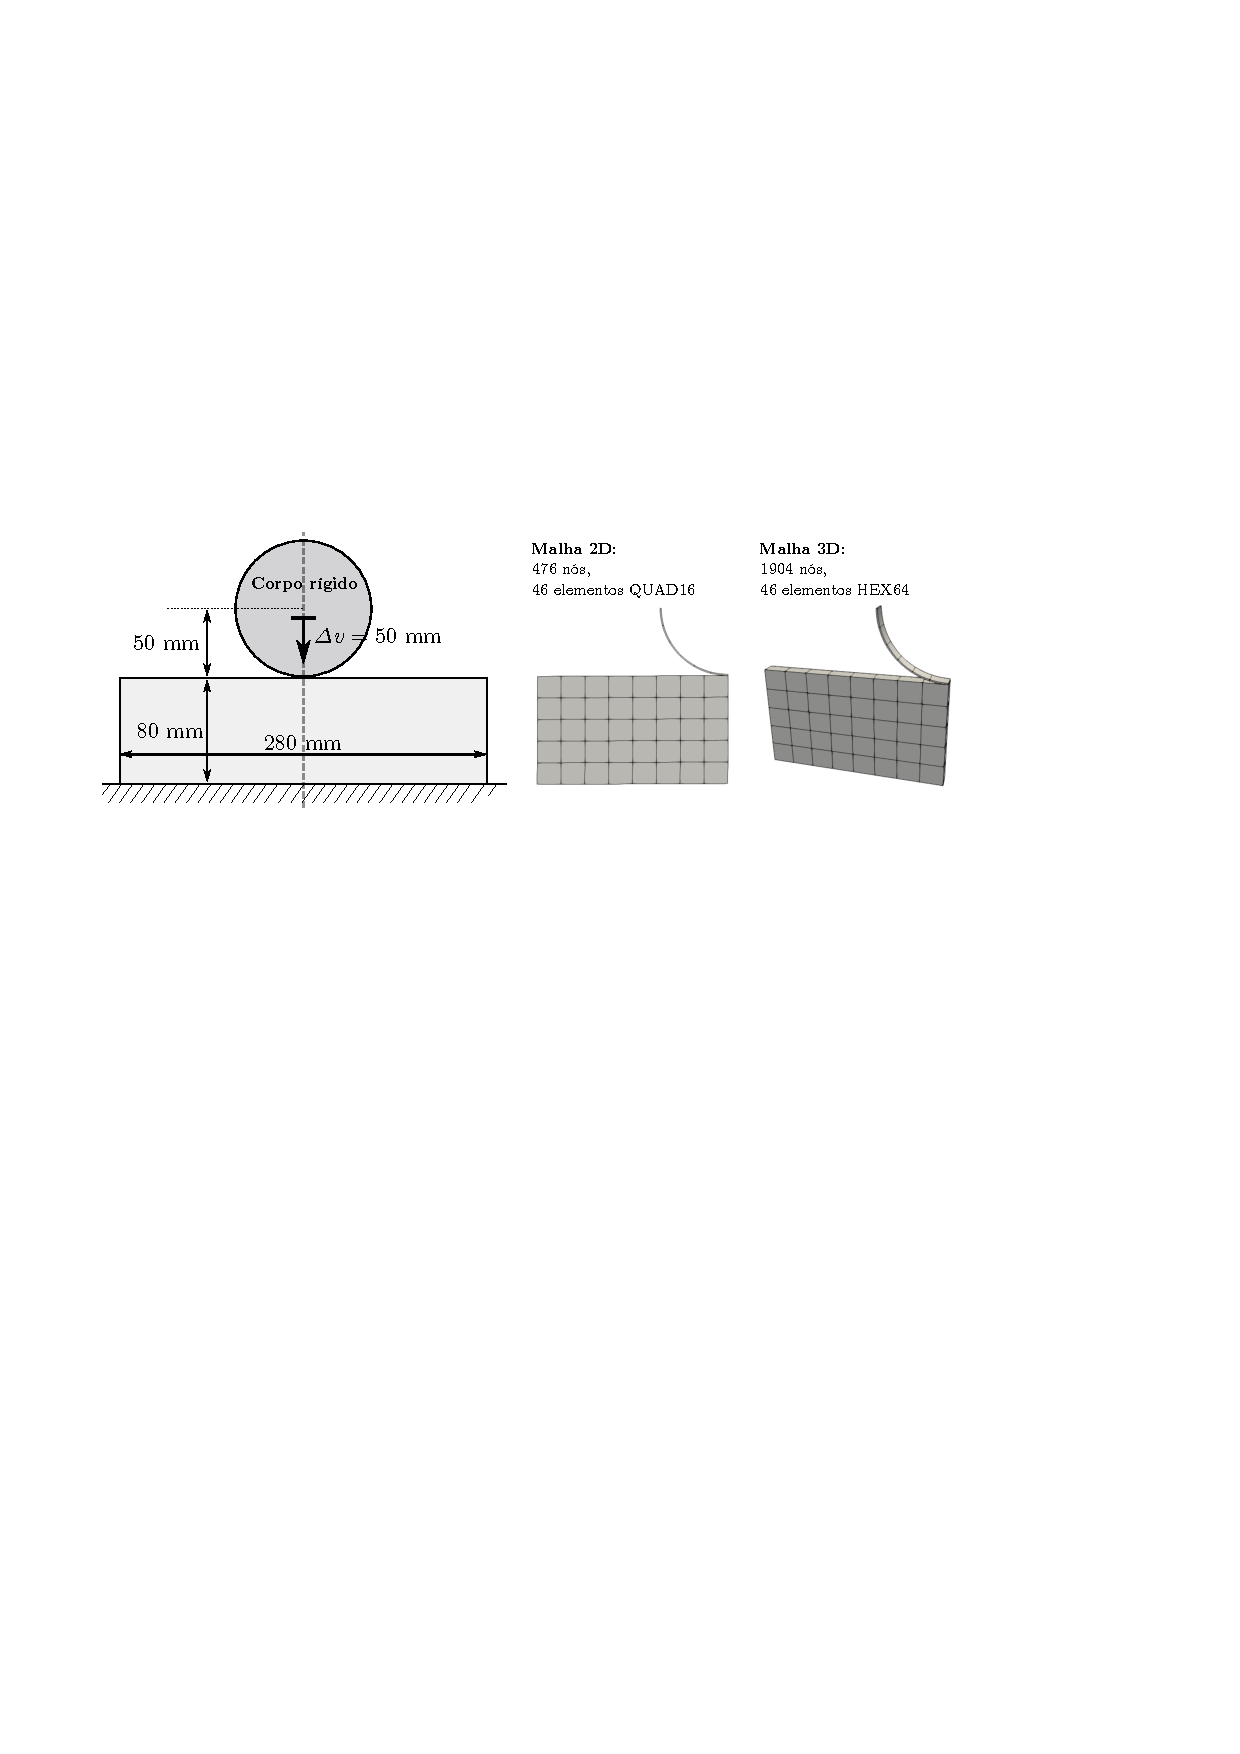
\includegraphics[scale=1.0]{Figuras/ExemplosContato/ExemploContato.pdf}\end{center}\par}
				\vspace{-0.2cm}
			}
		}
	}	
	%\caption*{\textbf{Fonte:} Elaborado pelo autor}
\end{figure}

De forma a permitir a concordância com o trabalho de \citeonline{FENG20032213}, utiliza-se neste exemplo em particular a lei hiperelástica de Blatz-Ko, onde temos $\S = \G\left(\J\C^{-1}-\C^{-2}\right)$, sendo considerado $G = 10$ N/mm$^2$.

Na \autoref{fig:exemploContatoResults}, são mostrados os resultados obtidos para os dois casos analisados. Na \autoref{fig:exemploContatoResults}(a), apresenta-se o gráfico de reação vertical total, onde observa-se uma excelente concordância com a referência em ambos os casos. Esses valores são tomados como a soma das forças de reação vertical em todos os nós do contorno inferior do bloco, multiplicado por dois para considerar a parte simétrica não discretizada do domínio. Por fim, nas Figuras \ref{fig:exemploContatoResults}(b) e \ref{fig:exemploContatoResults}(c) mostram-se as configurações deformadas do problema no último passo, para os casos 2D e 3D, respectivamente, com componentes $\cauchyind_{22}$ da tensão de Cauchy ilustradas em mapa de cores. Como esperado, os valores máximo e mínimo de tensão são consistentes entre os dois casos, apesar de se tratarem de análises em dimensões diferentes.


\begin{figure}[!htb]
	\centering
	\caption{Resultados do exemplo de contato entre cilindro e bloco hiperelástico, com (a) gráfico de força de reação vertical e configuração deformada final com componentes $\cauchyind_{22}$ de tensão de Cauchy em mapa de cores, para os casos (b) 2D e (c) 3D}
	\label{fig:exemploContatoResults}
	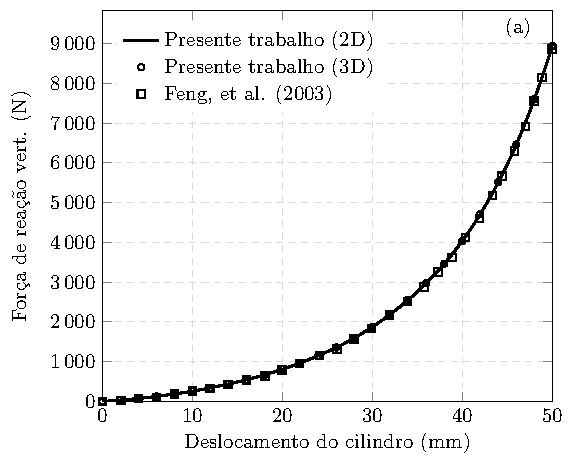
\includegraphics[scale=1.0]{Figuras/ExemplosContato/ExemploContatoReaction.pdf}\;\;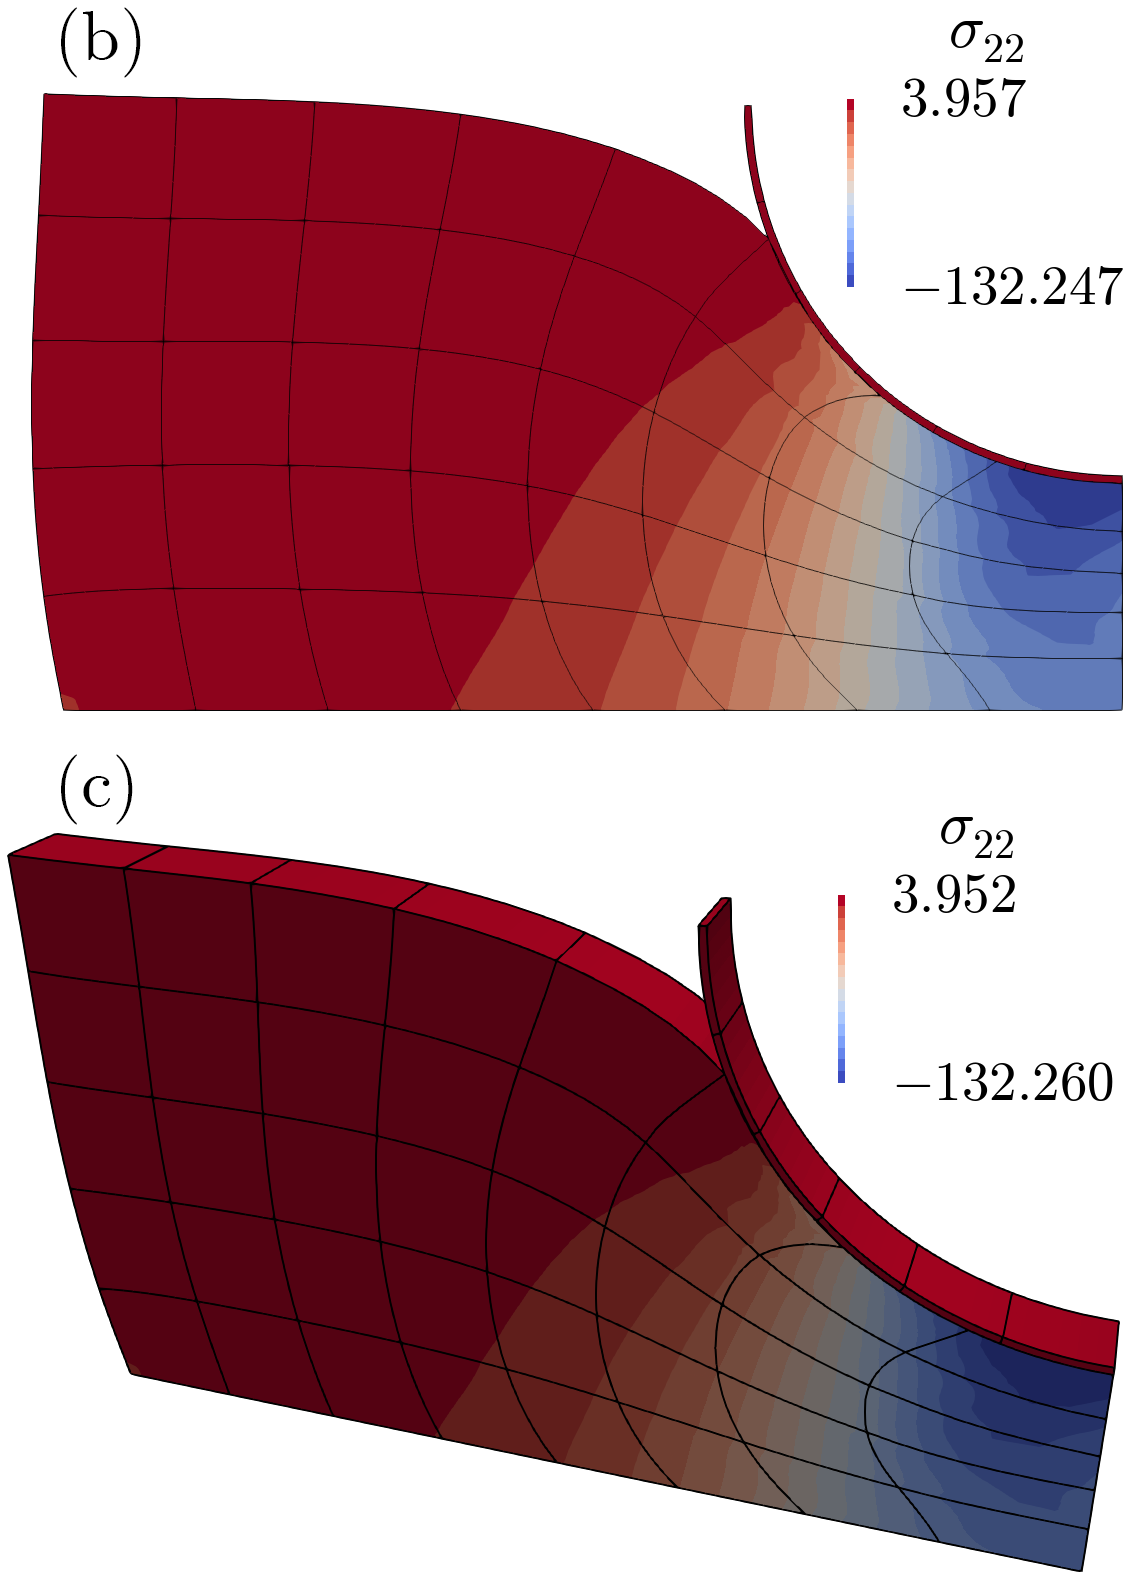
\includegraphics[scale=0.14]{Figuras/ExemplosContato/ExemploContatoResults2D3D.png}	
	%\caption*{\textbf{Fonte:} Elaborado pelo autor}
\end{figure}


\subsection{Contato entre esfera e bloco hiperelástico}\label{subsec:contatoEsfera}

Nesta seção, propõe-se uma versão intrinsecamente 3D do exemplo anterior, considerando o contato entre uma superfície rígida esférica e um bloco tridimensional, com geometria disposta na \autoref{fig:contatoEsfera}. Devido à simetria, apenas $1/4$ do exemplo é discretizado, sendo aplicadas as respectivas restrições nos eixos de simetria gerados. A malha utiliza $5120$ nós, e $150$ elementos hexaédricos de ordem 3 (HEX64). Novamente, considera-se a lei hiperelástica de Blatz-Ko para o bloco, com $G = 10$ N/mm$^2$, $100$ passos de tempo, e coeficiente de atrito $\friction = 0,4$.


\begin{figure}[!htb]
	\centering
	\caption{Dados do exemplo de contato entre esfera e bloco hiperelástico}
	\label{fig:contatoEsfera}
	{\small
		\noindent\shadowbox{
			\parbox{15.3cm}{
				\setlength{\columnseprule}{1pt}
				\vspace{-0.2cm}
				{\centering\begin{center}
				\includegraphics[scale=0.95]{Figuras/ExemplosContato/contatoEsfera.pdf}
				\end{center}\par}
				\vspace{-0.2cm}
			}
		}
	}	
	%\caption*{\textbf{Fonte:} Elaborado pelo autor}
\end{figure}

O gráfico de força de reação vertical para este caso é apresentado na \autoref{fig:contatoEsferaresults}(a), onde os valores são obtidos pela soma das forças de reação de cada nó na interface inferior do bloco, multiplicado por $4$ para considerar as parcelas simétricas não discretizadas. Além disso, apresenta-se na \autoref{fig:contatoEsferaresults}(b) a configuração deformada final do problema, isto é, a configuração no passo $100$, sendo indicadas as componentes $\cauchyind_{22}$ da tensão de Cauchy em mapa de cores.

\begin{figure}[!htb]
	\centering
	\caption{(a) Força de reação vertical e (b) configuração deformada final para exemplo de contato entre esfera e bloco hiperelástico}
	\label{fig:contatoEsferaresults}
	\includegraphics[scale=1.0]{Figuras/ExemplosContato/contatoEsferaReaction.pdf}\;\;\;\includegraphics[scale=0.235]{Figuras/ExemplosContato/contatoEsferaResultsB.png}
	%\caption*{\textbf{Fonte:} Elaborado pelo autor}
\end{figure}

\subsection{Contato entre lajes em balanço}\label{subsec:ExemplosContatoSlab}

Neste exemplo, propõe-se o contato sem atrito entre duas lajes em balanço, com geometria disposta na \autoref{fig:ExemplosContatoSlab}. Aplica-se deslocamento prescrito vertical em um dos apoios, evoluindo monotonicamente de $0$ a $-140$ cm em um total de $200$ passos de tempo. Com relação à malha, cada laje é discretizada em $64$ elementos hexaédricos de ordem 3 (HEX64). Por fim, o material adotado neste caso é neo-Hookeano, com $E = 1000$ kN/cm$^2$ e $\nu = 0,3$.

\begin{figure}[!htb]
	\centering
	\caption{Dados do exemplo de contato entre lajes}
	\label{fig:ExemplosContatoSlab}
	{\small
		\noindent\shadowbox{
			\parbox{15.3cm}{
				\setlength{\columnseprule}{1pt}
				\vspace{-0.2cm}
				{\centering\begin{center}
					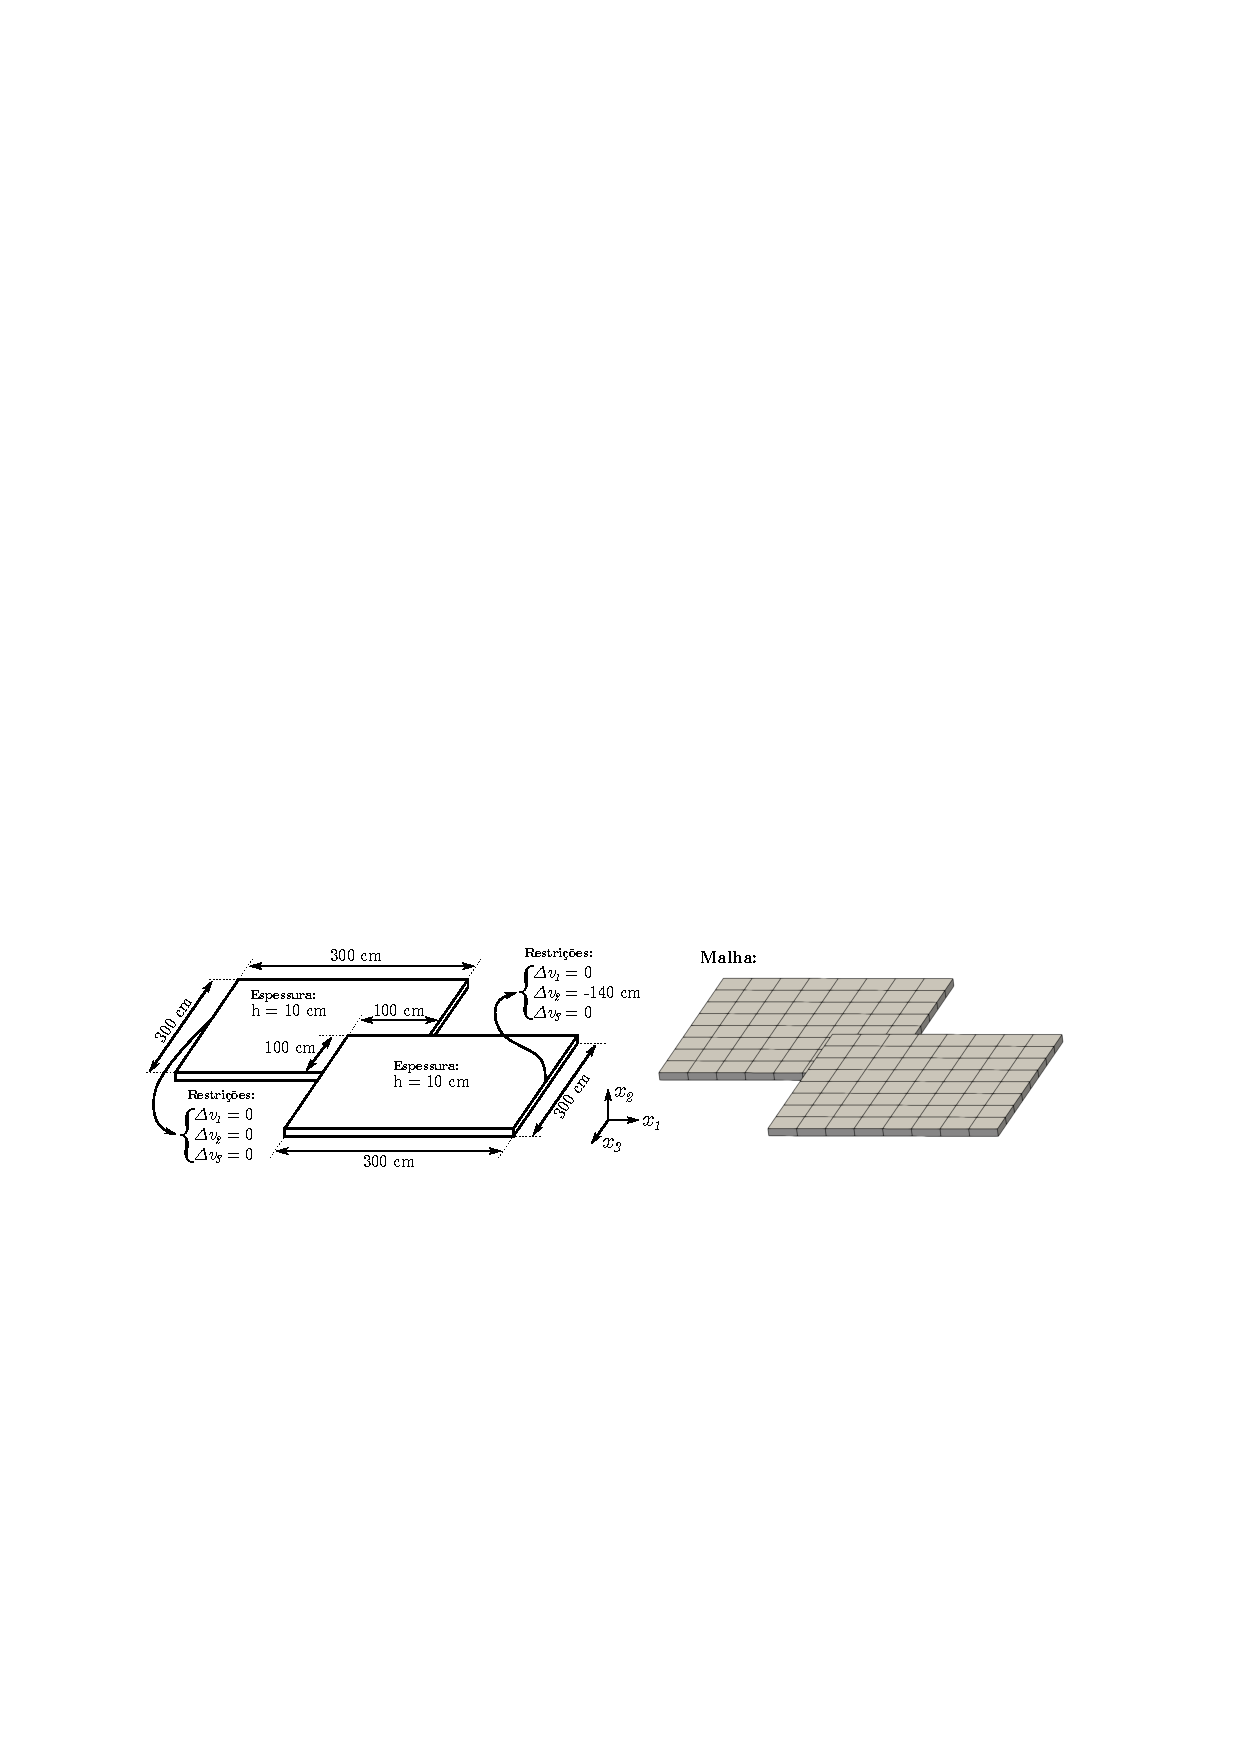
\includegraphics[scale=0.98]{Figuras/ExemplosContato/ExemplosContatoSlab.pdf}
					\end{center}\par}
				\vspace{-0.2cm}
			}
		}
	}	
	%\caption*{\textbf{Fonte:} Elaborado pelo autor}
\end{figure}

Na \autoref{fig:ExemplosContatoSlabResults} são apresentadas as configurações deformadas para os tempos $t=1/4$, $t=1/2$, $t=3/4$ (configurações intermediárias) e $t=1$ (configuração final), com mapas de cores indicando a componente horizontal da tensão de Cauchy, $\cauchyind_{11}$. Além disso, na \autoref{fig:ExemplosContatoSlabReactions} são mostradas as forças de reação no apoio onde é aplicado o deslocamento prescrito, tomadas, para cada caso, como a soma das forças em todos os nós do apoio. Observa-se que as reações no eixo $x_1$ e $x_3$ apresentam trechos de descontinuidade. Esses erros são esperados no presente algoritmo, uma vez que a ativação e desativação de nós de contato entre passos de tempo é um processo naturalmente descontínuo, mas podem ser reduzidos com o refinamento da malha.

\begin{figure}[!htb]
	\centering
	\caption{Configurações deformadas do exemplo de contato entre lajes para $4$ passos de tempo diferentes, com componente $\cauchyind_{11}$ da tensão de Cauchy em mapa de cores}
	\label{fig:ExemplosContatoSlabResults}
	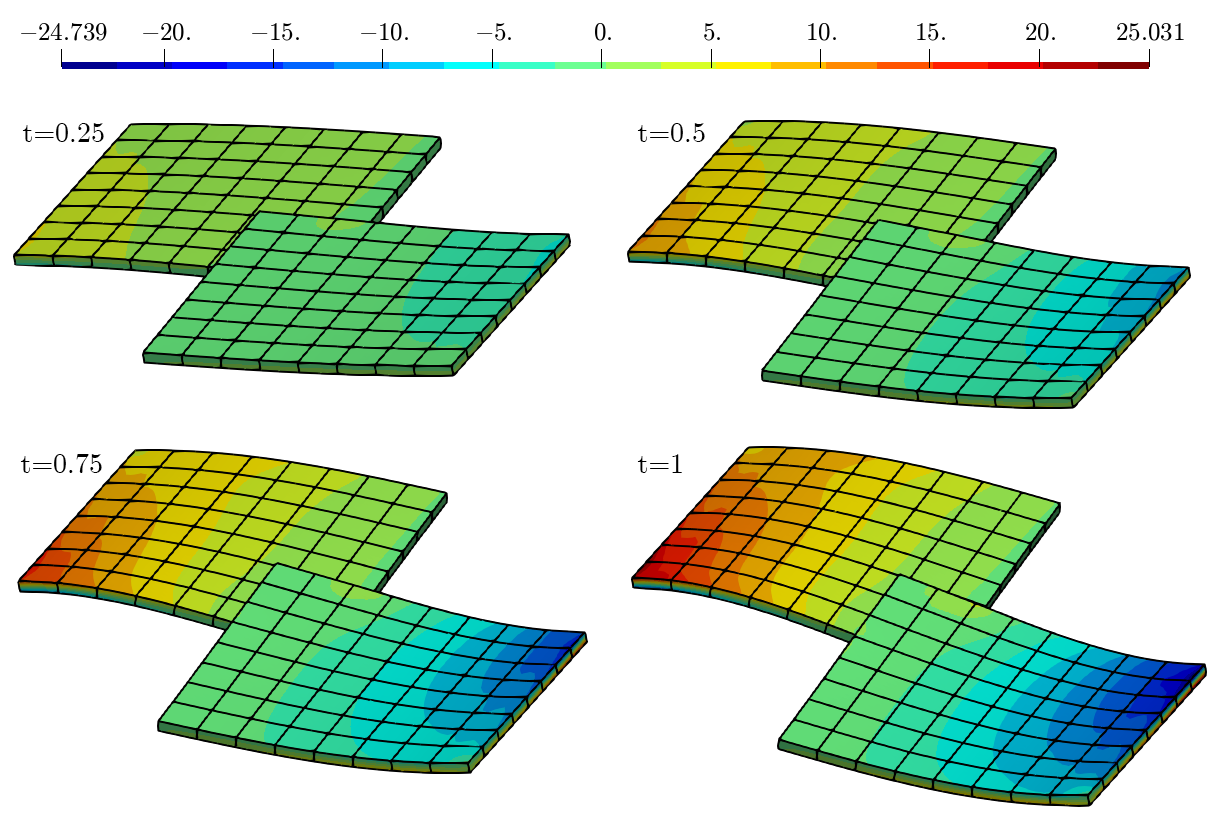
\includegraphics[scale=0.37]{Figuras/ExemplosContato/ContactSlabResults.png}
	%\caption*{\textbf{Fonte:} Elaborado pelo autor}
\end{figure}

\begin{figure}[!htb]
	\centering
	\caption{Gráficos reações de apoio nas direções (a) $x_2$, (b) $x_1$ e $x_3$ para o exemplo de contato entre lajes}
	\label{fig:ExemplosContatoSlabReactions}
	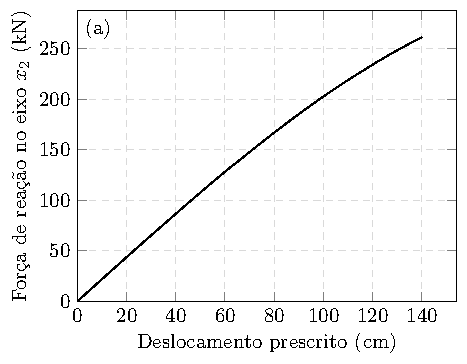
\includegraphics[scale=1.0]{Figuras/ExemplosContato/ContactSlabReactionY.pdf}\;\;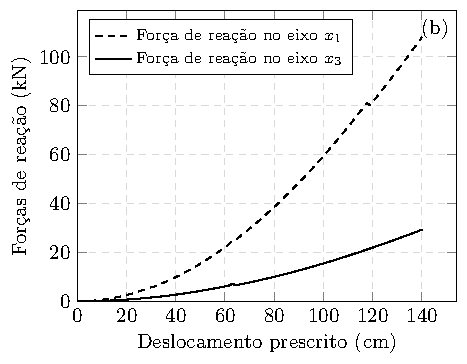
\includegraphics[scale=1.0]{Figuras/ExemplosContato/ContactSlabReactions.pdf}	
	%\caption*{\textbf{Fonte:} Elaborado pelo autor}
\end{figure}

\subsection{Dobramento simples de chapa metálica}\label{subsec:simple-bending}

Este exemplo é proposto originalmente em \citeonline{Pericles2019}, sendo reapresentado neste trabalho para mostrar as aplicações do algoritmo de contato implementado. Trata-se da simulação do processo de dobramento de uma chapa metálica retangular, que assume formato de L após ser impelida contra dois anteparos rígidos. Assume-se que as peças sejam suficientemente lubrificadas de forma a garantir que o atrito possa ser desprezado. Os dados do exemplo estão dispostos na \autoref{fig:simpleBending}, sendo novamente aproveitada a simetria para discretização do sólido.

\begin{figure}[!htb]
	\centering
	\caption{Dados do exemplo de dobramento simples de chapa metálica}
	\label{fig:simpleBending}
	{\small
		\noindent\shadowbox{
			\parbox{15.3cm}{
				\setlength{\columnseprule}{1pt}
				\vspace{-0.2cm}
				{\centering\begin{center}
					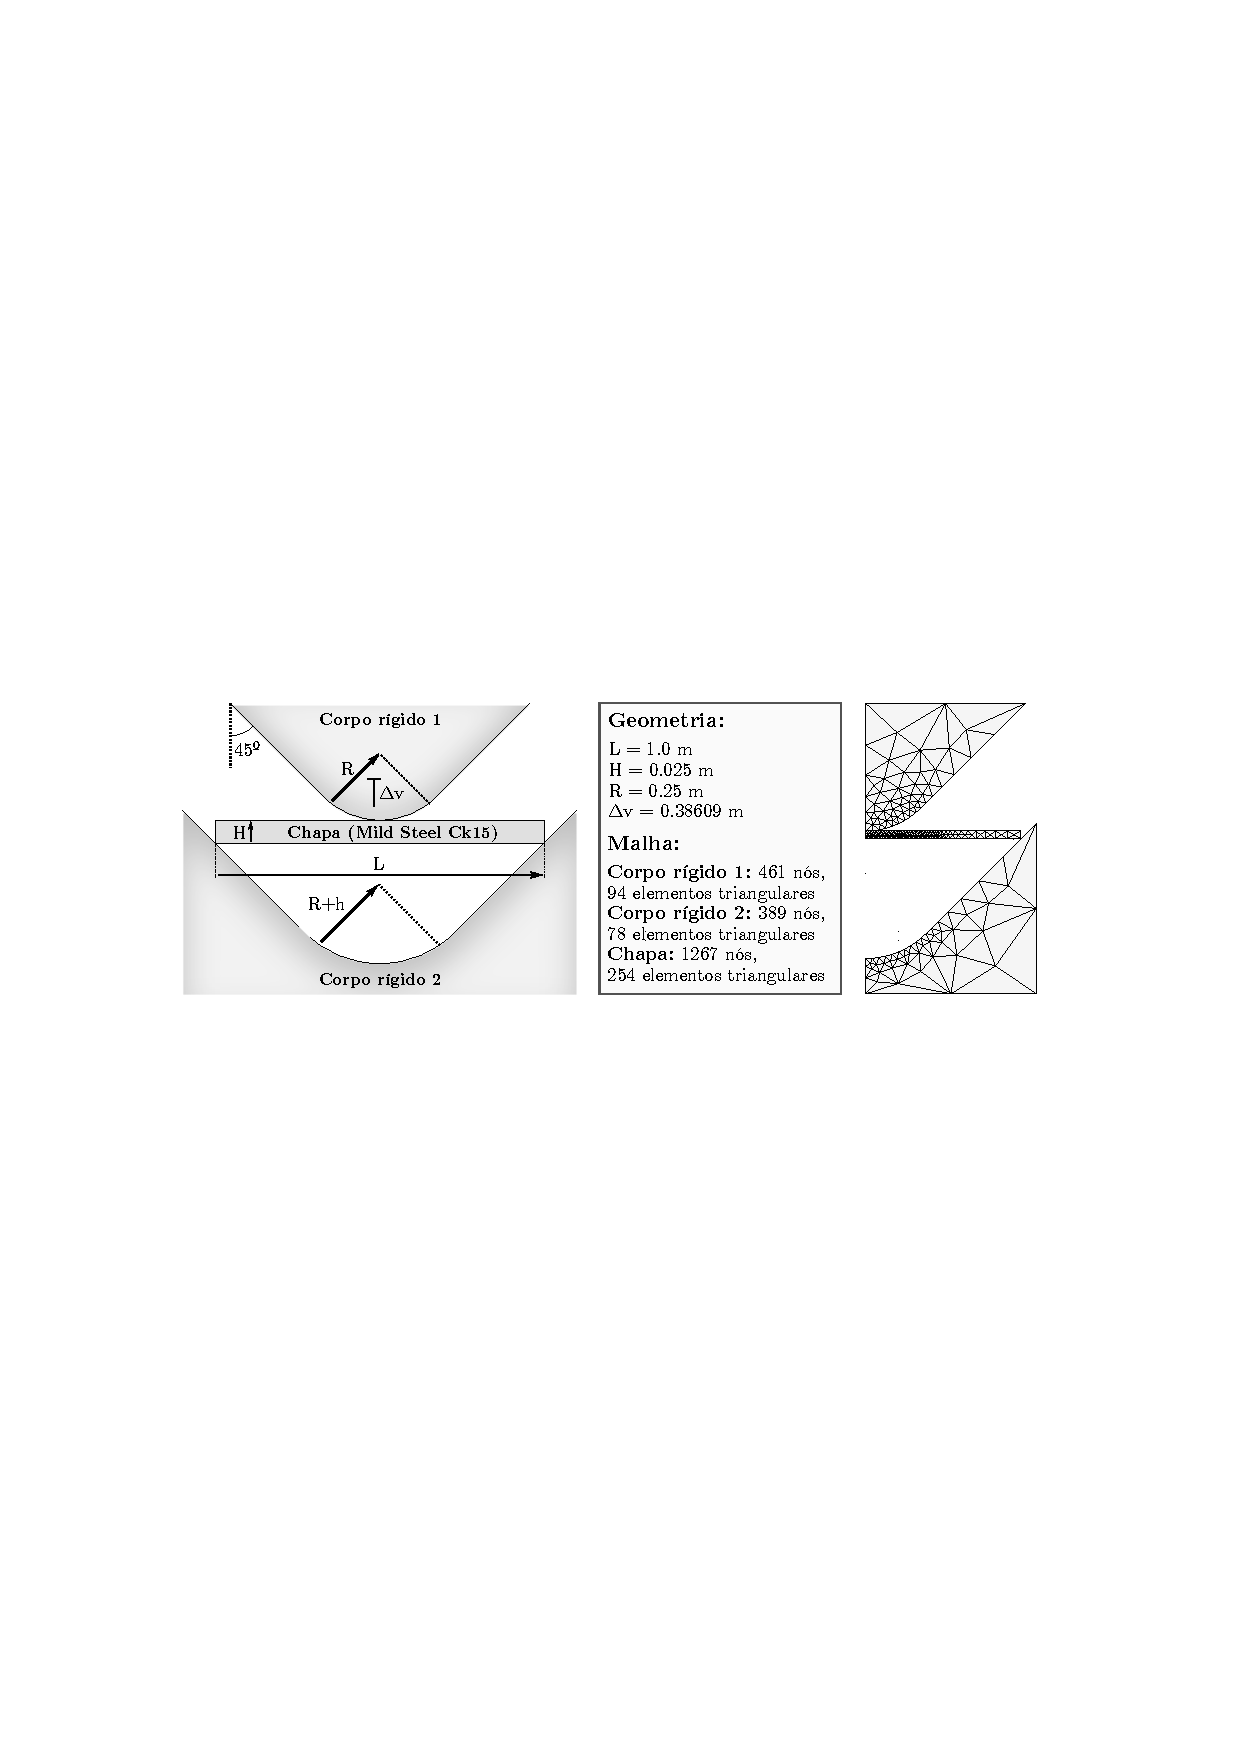
\includegraphics[scale=1.04]{Figuras/ExemplosContato/SimpleBending.pdf}
					\end{center}\par}
				\vspace{-0.2cm}
			}
		}
	}	
	%\caption*{\textbf{Fonte:} Elaborado pelo autor}
\end{figure}

Os blocos superior e inferior são simulados como corpos rígidos. Já para a chapa metálica considera-se o material \emph{Mild Steel Ck15}, simulado pelo modelo elasto-plástico em grandes deformações com encruamento cinemático de Armstrong-Frederick. Os parâmetros do modelo constitutivo são retirados do trabalho de \citeonline{HEERES20021}, e apresentados na \autoref{tab:mildsteelck15}.

\begin{table}[h]
	\centering
	\caption{Parâmetros do material \emph{Mild Steel Ck15}, retirados de \citeonline{HEERES20021}}
	\label{tab:mildsteelck15}
	{\tabulinesep=1.5mm
		\begin{tabu}{ccccc}
			\hline
			\rowcolor{LightGray}
			$\lamee$ (MPa) & $\Ge$ (MPa) & $\yieldStresscte$ (MPa) & $\armstrongstiff$ (MPa) & $\armstrongvisc$ \\ \hline
			$173\,333$ & $80\,000$ & $300$ & $1\,900$ & $8,5$ \\ \hline	
		\end{tabu}	
	}
	%\caption*{\textbf{Fonte:} Elaborado pelo autor}
\end{table}

O processo de dobramento é simulado em 3000 passos de deslocamento prescrito. Em seguida, aplica-se mais um passo de retirada do anteparo rígido, para que possa ser observado o recuo (\emph{Springback}) manifestado na chapa metálica. As configurações deformadas de alguns passos chaves da análise são mostradas na \autoref{fig:simpleBendingResults}, incluindo a configuração final após a retirada da peça. Foi obtido um ângulo final da chapa metálica de aproximadamente $92,12^{\circ}$, isto é, houve, após o \emph{Springback}, uma variação de $0,88^{\circ}$ com relação ao ângulo imposto de $90^{\circ}$. 

\begin{figure}[!htb]
	\centering
	\caption{Configurações deformadas para o exemplo de dobramento simples de chapa metálica, com componentes horizontais de deformação plástica, $(\Epind)_{11}$ ilustradas em mapas de cores}
	\label{fig:simpleBendingResults}
	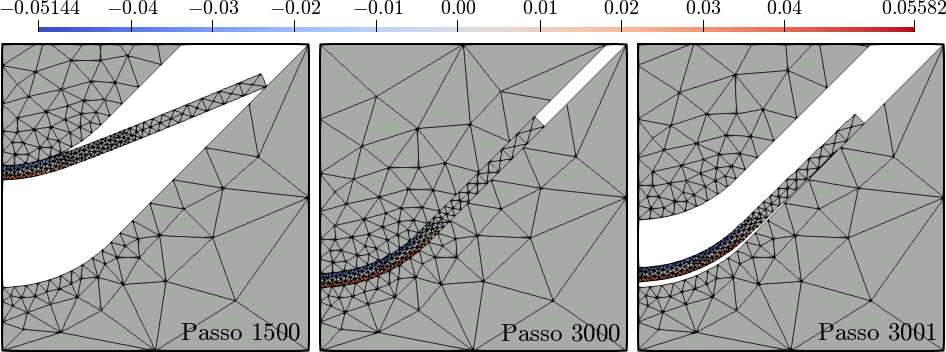
\includegraphics[scale=0.47]{Figuras/ExemplosContato/SimpleBendingResults.png}
	\caption*{\textbf{Fonte:} \citeonline{Pericles2019}}
\end{figure}

\subsection{Dobramento direcionado (\emph{draw bending}) de barra metálica}\label{subsec:draw-bending}

Neste exemplo é feita uma simulação numérica do processo de dobramento direcionado, apresentado como alternativa ao dobramento simples (exemplo anterior) para a obtenção de um mesmo formato de peça. Este exemplo é proposto originalmente em \citeonline{Pericles2019} para o caso sem atrito, e foi estendido neste texto para o caso com atrito, considerando os coeficientes $\friction = 0,05$ e $\friction = 0,1$. Os dados de geometria e condição de contorno são apresentados na \autoref{fig:drawBending}. Novamente, considera-se o material \emph{Mild Steel Ck15} para a chapa, cujos parâmetros são dados na \autoref{tab:mildsteelck15}. O processo de dobramento é feito em $3000$ passos de deslocamento prescrito, seguidos de $1$ passo onde os anteparos rígidos são removidos, para demonstrar o efeito do \emph{Springback}.

\begin{figure}[!htb]
	\centering
	\caption{Dados do exemplo de dobramento direcionado (\emph{draw bending}) de barra metálica}
	\label{fig:drawBending}
	{\small
		\noindent\shadowbox{
			\parbox{15.3cm}{
				\setlength{\columnseprule}{1pt}
				\vspace{-0.2cm}
				{\centering\begin{center}
					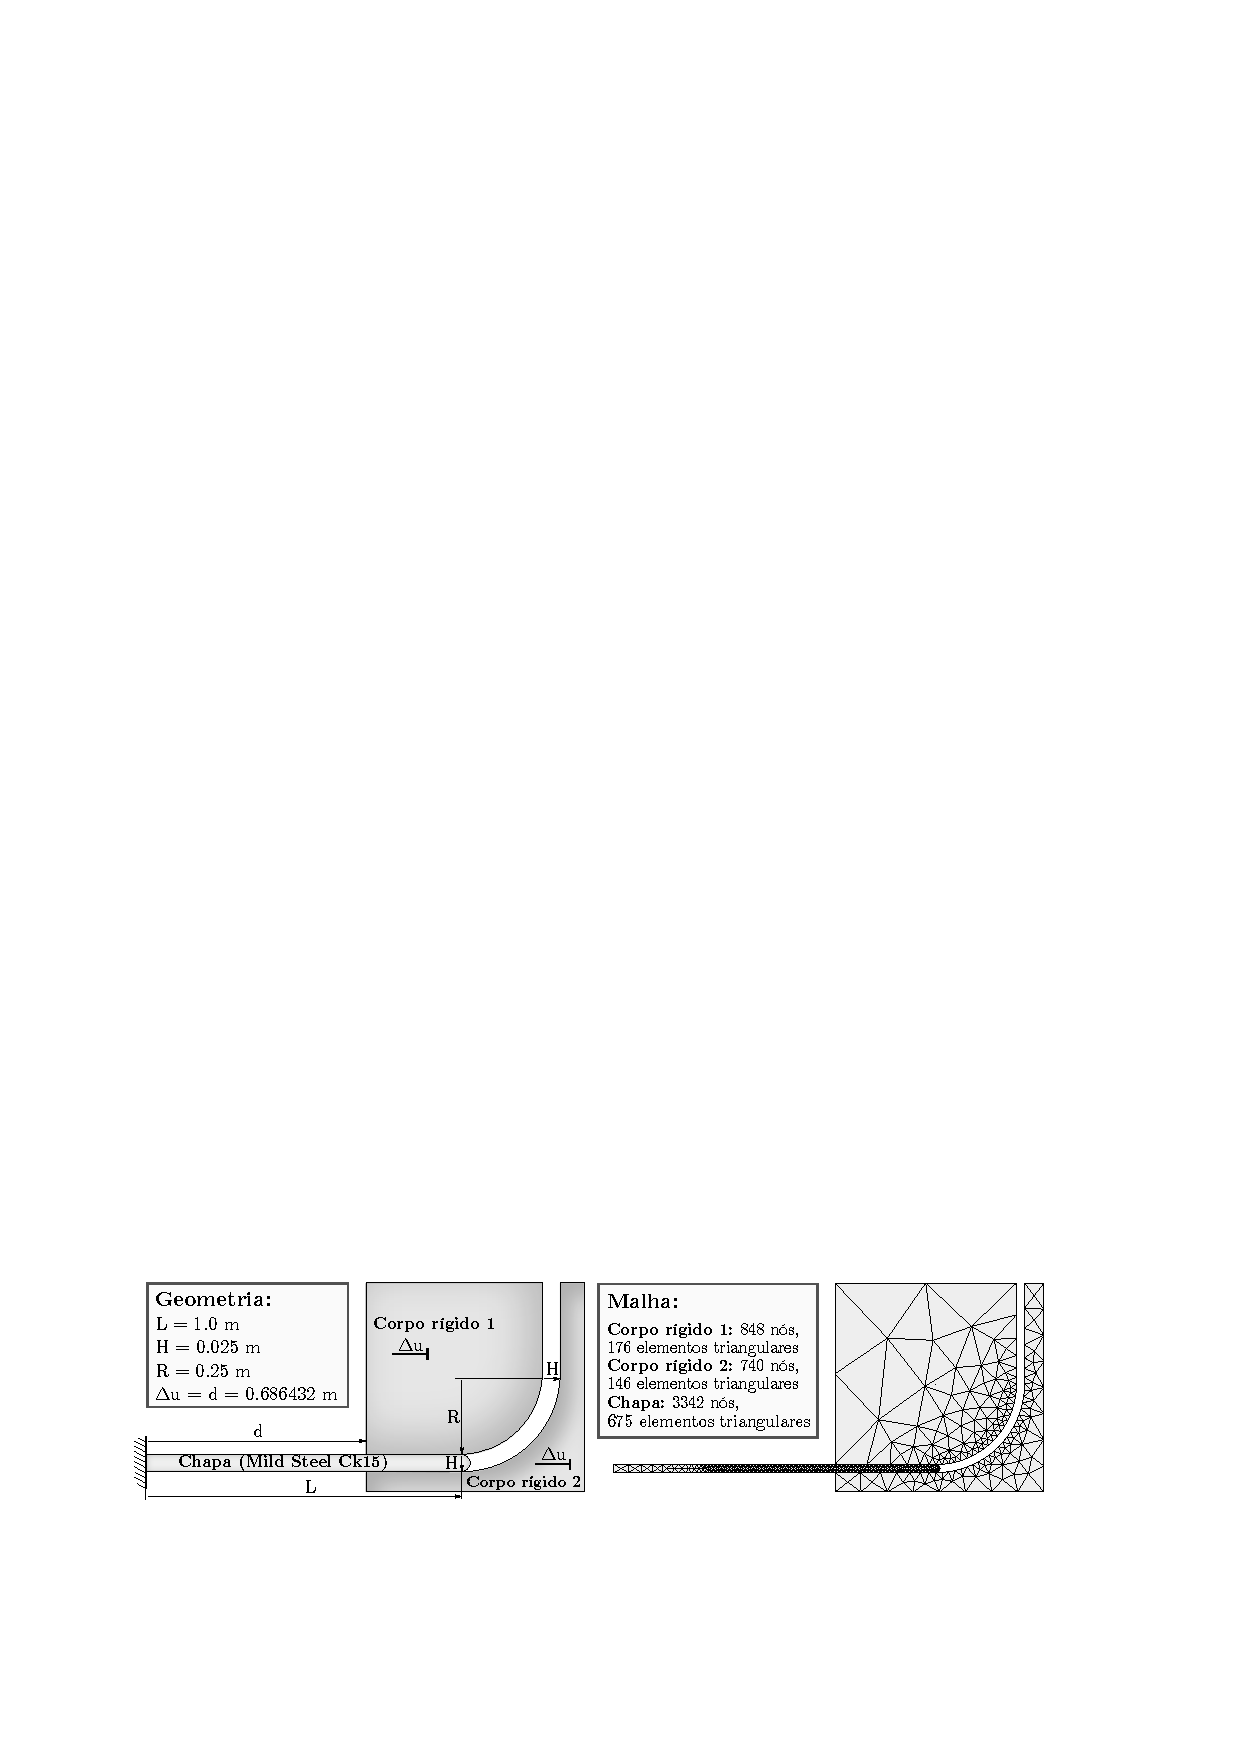
\includegraphics[scale=0.98]{Figuras/ExemplosContato/DrawBending.pdf}
					\end{center}\par}
				\vspace{-0.2cm}
			}
		}
	}	
	%\caption*{\textbf{Fonte:} Elaborado pelo autor}
\end{figure}


A principal diferença do dobramento direcionado com relação ao dobramento simples é o fato de que algumas regiões da peça são sujeitas ao dobramento seguido de retificação, ativando o efeito de \emph{Bauschinger}. As consequências desse efeito podem ser vistas na \autoref{fig:drawBendingResults}, onde apresentam-se as configurações deformadas e a componente $(\Epind)_{11}$ das deformações plásticas para o caso sem atrito. Como pode ser visto, ao contrário do exemplo anterior, neste caso as deformações plásticas não se concentram apenas na região central da peça, mas também residualmente na região superior, onde houve anteriormente o processo de dobramento.

\begin{figure}[!htb]
	\centering
	\caption{Configurações deformadas do exemplo de dobramento direcionado para o caso sem atrito, apresentando a componente $(\Epind)_{11}$ das deformações plásticas em mapa de cores}
	\label{fig:drawBendingResults}
	\includegraphics[scale=0.45]{Figuras/ExemplosContato/drawBendingResults.png}
	%\caption*{\textbf{Fonte:} Elaborado pelo autor}
\end{figure}

\begin{figure}[!b]
	\centering
	\caption{Configurações deformadas finais do exemplo de dobramento direcionado para os três casos de atrito, apresentando a componente $(\Epind)_{11}$ das deformações plásticas em mapa de cores}
	\label{fig:drawBendingResults2}
	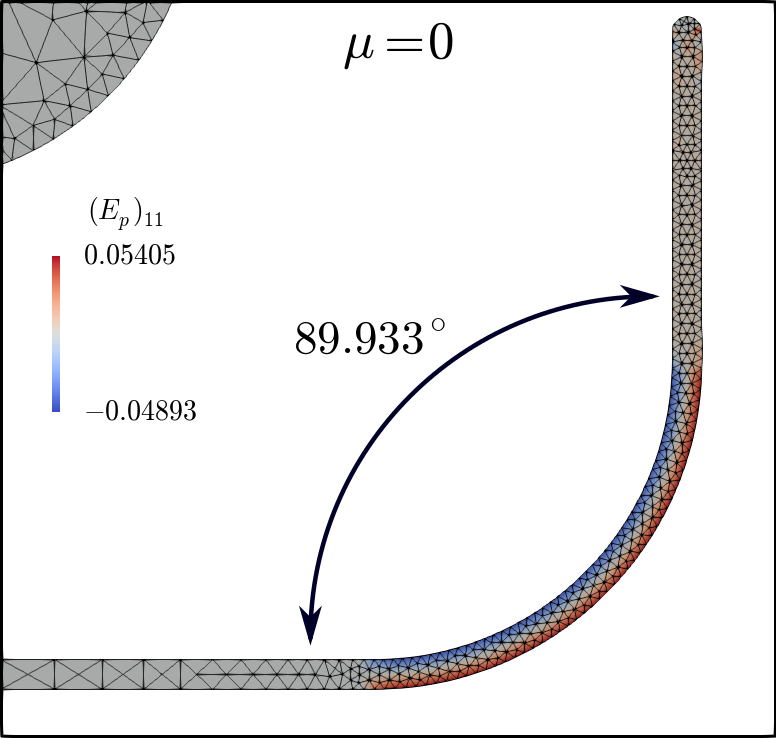
\includegraphics[scale=0.19]{Figuras/ExemplosContato/DrawBending-mu0.png}\;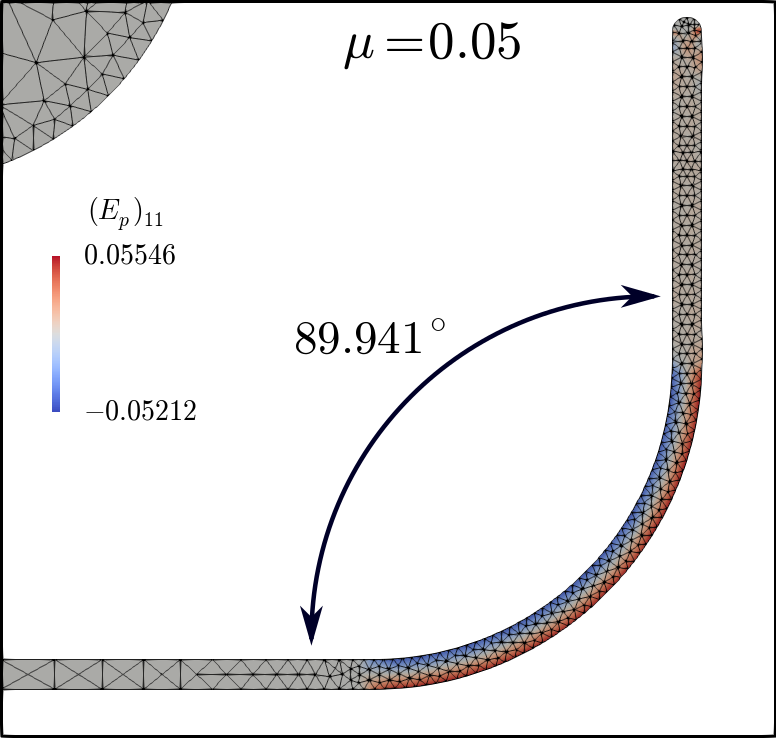
\includegraphics[scale=0.19]{Figuras/ExemplosContato/DrawBending-mu005.png}\;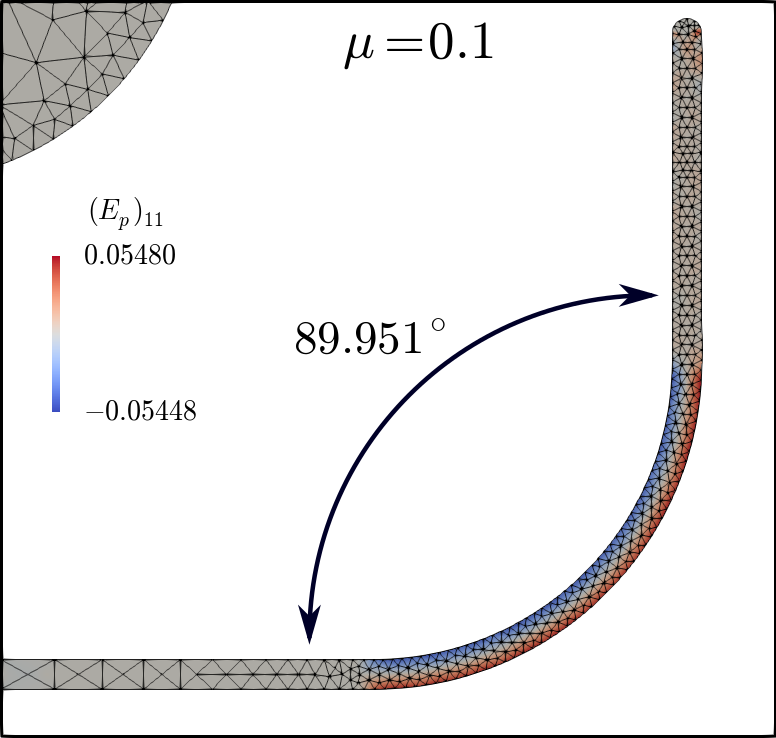
\includegraphics[scale=0.19]{Figuras/ExemplosContato/DrawBending-mu01.png}
	%\caption*{\textbf{Fonte:} Elaborado pelo autor}
\end{figure}

Como consequência, o exemplo de dobramento direcionado apresenta diferenças na sua configuração deformada final com relação ao dobramento simples: o ângulo obtido para a chapa neste caso é menor que 90$^{\circ}$, como pode ser visto na \autoref{fig:drawBendingResults2}. Este ângulo varia de acordo com o coeficiente de atrito utilizado, porém, em todos os casos ele é bem mais próximo de 90$^{\circ}$ do que o ângulo obtido no exemplo de dobramento simples, o que indica uma conformação mais adequada ao formato desejado. Observa-se ainda que a diferença provocada pelo coeficiente de atrito possui influência mínima na configuração deformada. No entanto, conforme apresentado na \autoref{fig:drawBending-Reaction}, este influencia altamente na reação de apoio horizontal, isto é, a força necessária para realizar o processo de dobramento direcionado (medida na extremidade esquerda da chapa).



\begin{figure}[!htb]
	\centering
	\caption{Gráficos de força de reação horizontal do exemplo de dobramento direcionado para os três casos de atrito}
	\label{fig:drawBending-Reaction}
	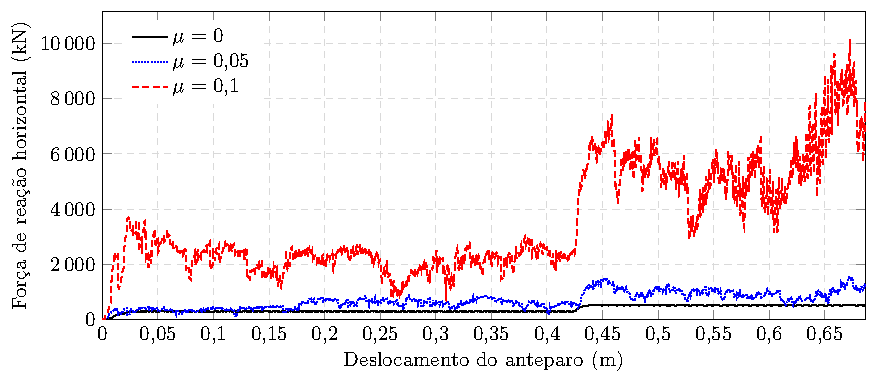
\includegraphics[scale=1.0]{Figuras/ExemplosContato/DrawBending-Reaction-pt.pdf}
	%\caption*{\textbf{Fonte:} Elaborado pelo autor}
\end{figure}

\subsection{Extrusão}\label{subsec:extrusion}

Assim como os exemplos anteriores, este é originalmente proposto em \citeonline{Pericles2019} para o caso sem atrito, sendo estendido neste texto para o caso com atrito, considerando os coeficientes $\friction=0,05$ e $\friction=0,1$. Trata-se de uma chapa metálica com material \emph{Mild Steel Ck15} (\autoref{tab:mildsteelck15}), compelida entre anteparos rígidos de formato circular, a fim de reduzir a altura da sua seção transversal em aproximadamente $30\%$. Dada a simetria do problema, apenas a parte superior foi discretizada, sendo aplicada as devidas condições de contorno no eixo de simetria. Os dados de geometria e malha são apresentados na \autoref{fig:extrusion}.

\begin{figure}[!htb]
	\centering
	\caption{Dados do exemplo de extrusão}
	\label{fig:extrusion}
	{\small
		\noindent\shadowbox{
			\parbox{15.3cm}{
				\setlength{\columnseprule}{1pt}
				\vspace{-0.2cm}
				{\centering\begin{center}
					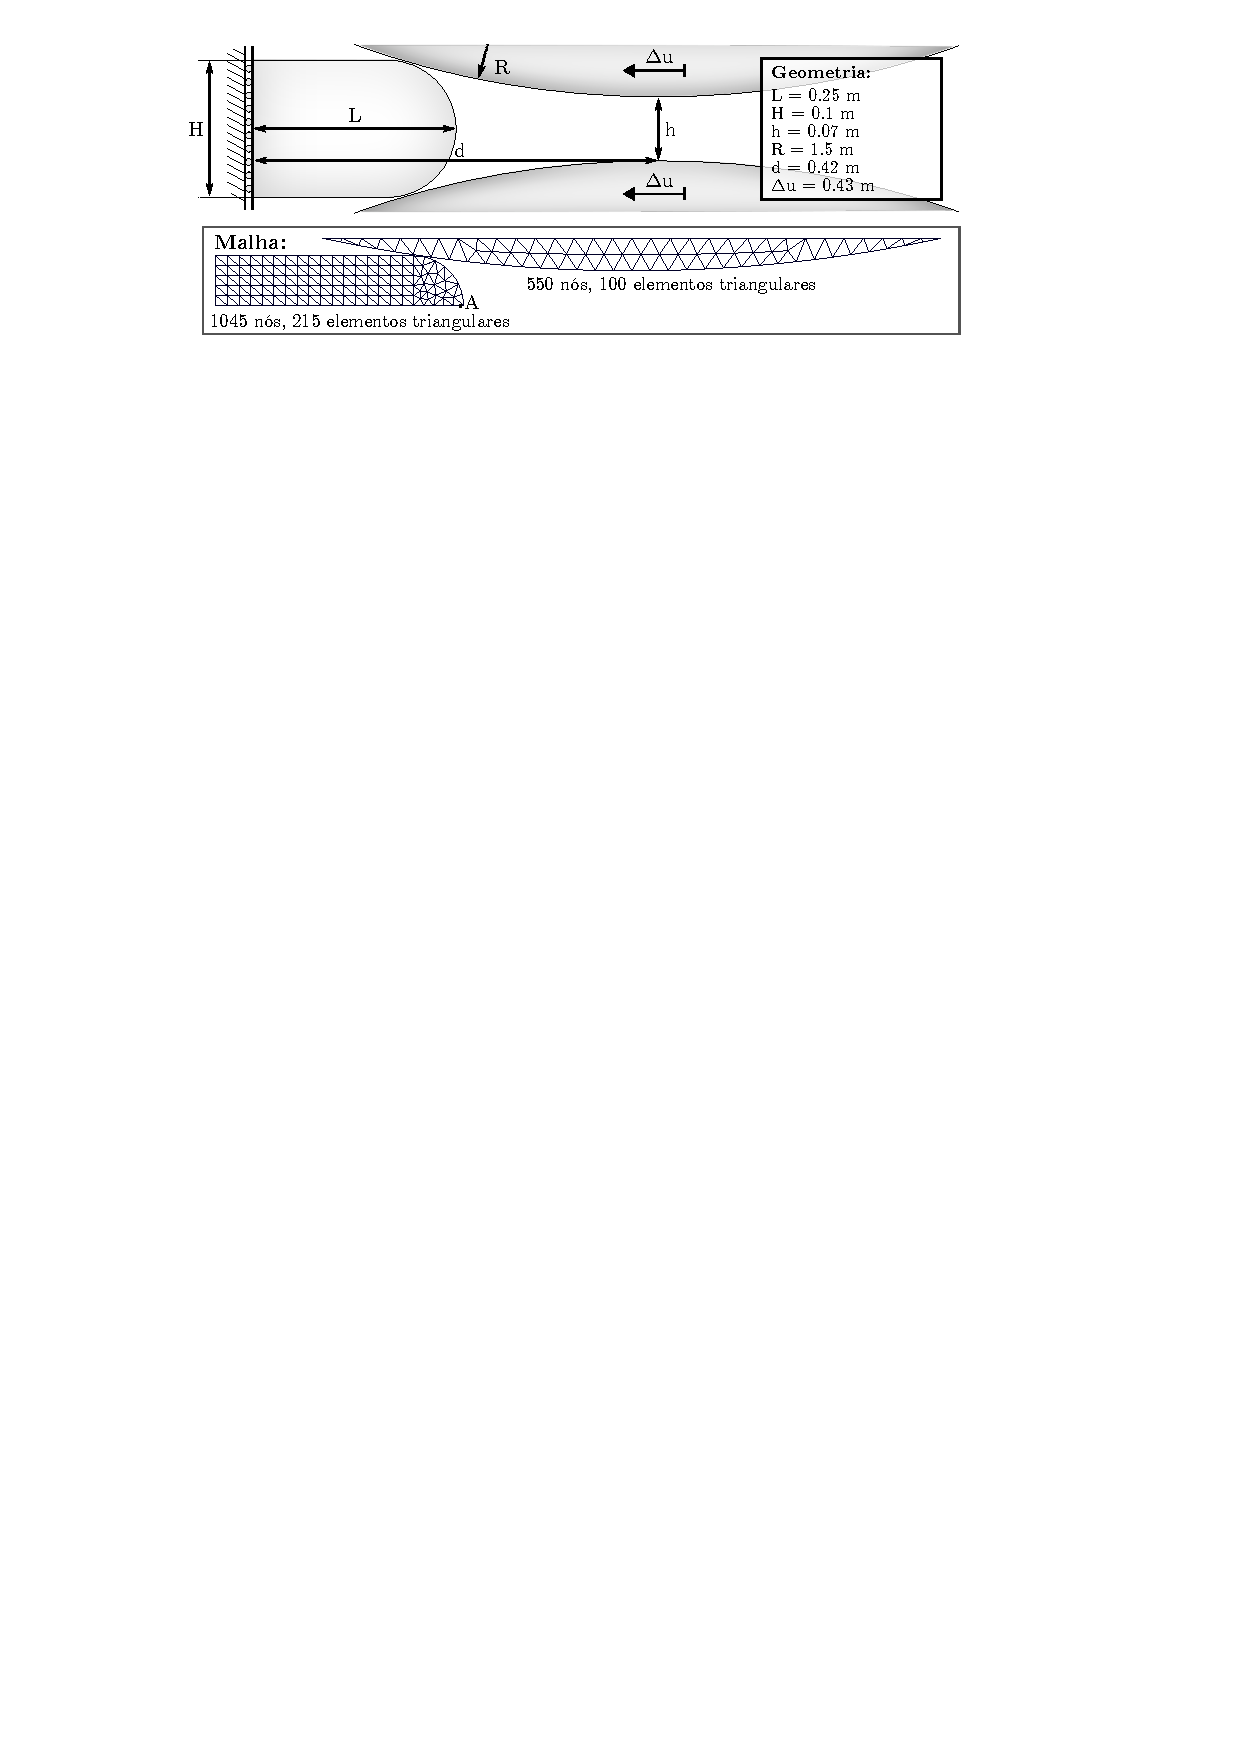
\includegraphics[scale=1.1]{Figuras/ExemplosContato/Extrusion.pdf}
					\end{center}\par}
				\vspace{-0.2cm}
			}
		}
	}	
	%\caption*{\textbf{Fonte:} Elaborado pelo autor}
\end{figure}

O processo foi simulado em uma análise estática com $8000$ passos de deslocamento prescrito, e utilizou-se estado plano de deformação para a chapa metálica. As configurações deformadas em diversos passos de tempo são mostradas para o caso sem atrito na \autoref{fig:Extrusion-Results0} e para o caso com coeficiente de atrito $\friction=0,1$ na \autoref{fig:Extrusion-Results01}. Embora a configuração deformada final seja aproximadamente igual para os dois casos no que diz respeito ao formato da peça, observa-se que a disposição das variáveis internas muda consideravelmente de um caso para o outro.

\begin{figure}[!htb]
	\centering
	\caption{Configurações deformadas do exemplo de extrusão sem atrito, apresentando a componente $(\Epind)_{11}$ das deformações plásticas em mapa de cores}
	\label{fig:Extrusion-Results0}
	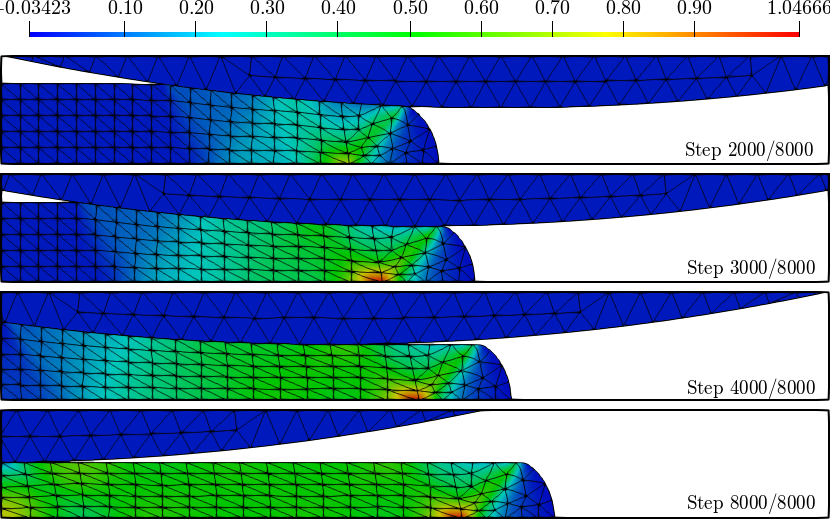
\includegraphics[scale=0.45]{Figuras/ExemplosContato/ExtrusionResults.png}
	%\caption*{\textbf{Fonte:} Elaborado pelo autor}
\end{figure}

\begin{figure}[!htb]
	\centering
	\caption{Configurações deformadas do exemplo de extrusão com $\friction = 0,1$, apresentando a componente $(\Epind)_{11}$ das deformações plásticas em mapa de cores}
	\label{fig:Extrusion-Results01}
	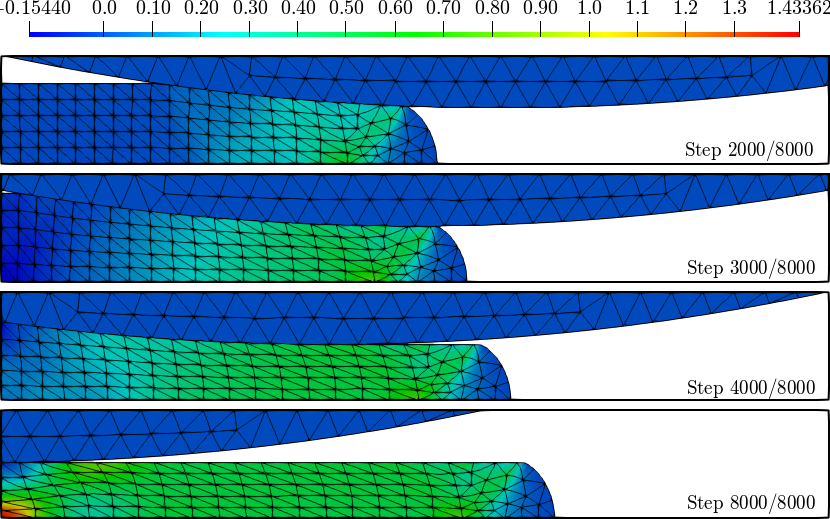
\includegraphics[scale=0.45]{Figuras/ExemplosContato/ExtrusionResults-Friction.png}
	%\caption*{\textbf{Fonte:} Elaborado pelo autor}
\end{figure}

Na \autoref{fig:Extrusion-Reaction} apresentam-se, por fim, os gráficos de reação horizontal total da chapa e deslocamento no ponto A ao longo do processo. O primeiro, mostrado na \autoref{fig:Extrusion-Reaction}(a), é calculado a partir da soma das forças internas horizontais de todos os nós do apoio na extremidade esquerda, multiplicada por $2$ de forma a considerar a parcela não discretizada do problema. Neste, observa-se uma alta influência do coeficiente de atrito, conforme esperado. Já o deslocamento no ponto A, mostrado na \autoref{fig:Extrusion-Reaction}(b), apresenta diferenças notáveis apenas no meio do processo, resultando no fim em valores praticamente equivalentes para os três casos.

\begin{figure}[!htb]
	\centering
	\caption{Gráficos de (a) força de reação horizontal e (b) deslocamento no ponto A para o exemplo de extrusão}
	\label{fig:Extrusion-Reaction}
	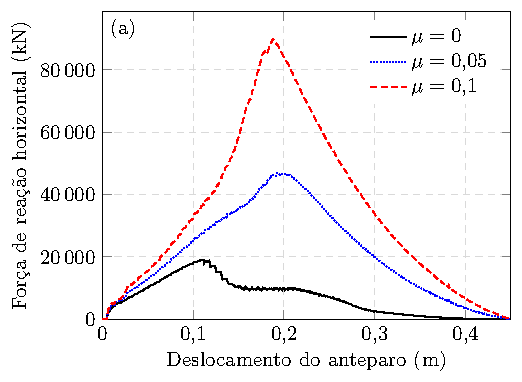
\includegraphics[scale=0.9]{Figuras/ExemplosContato/Extrusion-reaction-pt.pdf}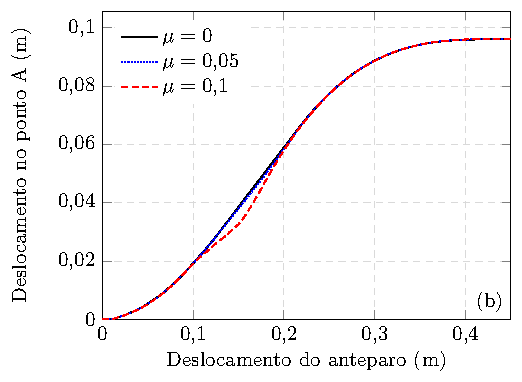
\includegraphics[scale=0.9]{Figuras/ExemplosContato/Extrusion-dispA-pt.pdf}
	%\caption*{\textbf{Fonte:} Elaborado pelo autor}
\end{figure}


\newpage
\null
\vfill

\end{document}
	
	
